% Options for packages loaded elsewhere
\PassOptionsToPackage{unicode}{hyperref}
\PassOptionsToPackage{hyphens}{url}
%
\documentclass[
  11pt,
]{article}
\usepackage{amsmath,amssymb}
\usepackage{iftex}
\ifPDFTeX
  \usepackage[T1]{fontenc}
  \usepackage[utf8]{inputenc}
  \usepackage{textcomp} % provide euro and other symbols
\else % if luatex or xetex
  \usepackage{unicode-math} % this also loads fontspec
  \defaultfontfeatures{Scale=MatchLowercase}
  \defaultfontfeatures[\rmfamily]{Ligatures=TeX,Scale=1}
\fi
\usepackage{lmodern}
\ifPDFTeX\else
  % xetex/luatex font selection
  \setmainfont[]{Times New Roman}
\fi
% Use upquote if available, for straight quotes in verbatim environments
\IfFileExists{upquote.sty}{\usepackage{upquote}}{}
\IfFileExists{microtype.sty}{% use microtype if available
  \usepackage[]{microtype}
  \UseMicrotypeSet[protrusion]{basicmath} % disable protrusion for tt fonts
}{}
\makeatletter
\@ifundefined{KOMAClassName}{% if non-KOMA class
  \IfFileExists{parskip.sty}{%
    \usepackage{parskip}
  }{% else
    \setlength{\parindent}{0pt}
    \setlength{\parskip}{6pt plus 2pt minus 1pt}}
}{% if KOMA class
  \KOMAoptions{parskip=half}}
\makeatother
\usepackage{xcolor}
\usepackage[margin=1in]{geometry}
\usepackage{graphicx}
\makeatletter
\def\maxwidth{\ifdim\Gin@nat@width>\linewidth\linewidth\else\Gin@nat@width\fi}
\def\maxheight{\ifdim\Gin@nat@height>\textheight\textheight\else\Gin@nat@height\fi}
\makeatother
% Scale images if necessary, so that they will not overflow the page
% margins by default, and it is still possible to overwrite the defaults
% using explicit options in \includegraphics[width, height, ...]{}
\setkeys{Gin}{width=\maxwidth,height=\maxheight,keepaspectratio}
% Set default figure placement to htbp
\makeatletter
\def\fps@figure{htbp}
\makeatother
\setlength{\emergencystretch}{3em} % prevent overfull lines
\providecommand{\tightlist}{%
  \setlength{\itemsep}{0pt}\setlength{\parskip}{0pt}}
\setcounter{secnumdepth}{-\maxdimen} % remove section numbering
\usepackage{setspace}
\doublespacing
\ifLuaTeX
  \usepackage{selnolig}  % disable illegal ligatures
\fi
\IfFileExists{bookmark.sty}{\usepackage{bookmark}}{\usepackage{hyperref}}
\IfFileExists{xurl.sty}{\usepackage{xurl}}{} % add URL line breaks if available
\urlstyle{same}
\hypersetup{
  pdftitle={71point4 Analyst Assignment},
  pdfauthor={André le Roux},
  hidelinks,
  pdfcreator={LaTeX via pandoc}}

\title{71point4 Analyst Assignment}
\author{André le Roux}
\date{2024-08-20}

\begin{document}
\maketitle

\hypertarget{introduction}{%
\section{Introduction}\label{introduction}}

This is the introduction section where you can provide an overview of
your analysis.

\hypertarget{question-3}{%
\subsection{Question 3}\label{question-3}}

I was unsure of the level of difficulty that the question should be, so
I decided to go for a question with two part that can given individually
or together.

\hypertarget{part-a}{%
\subparagraph{Part A}\label{part-a}}

\hypertarget{graph-4.1}{%
\subsection{Graph 4.1}\label{graph-4.1}}

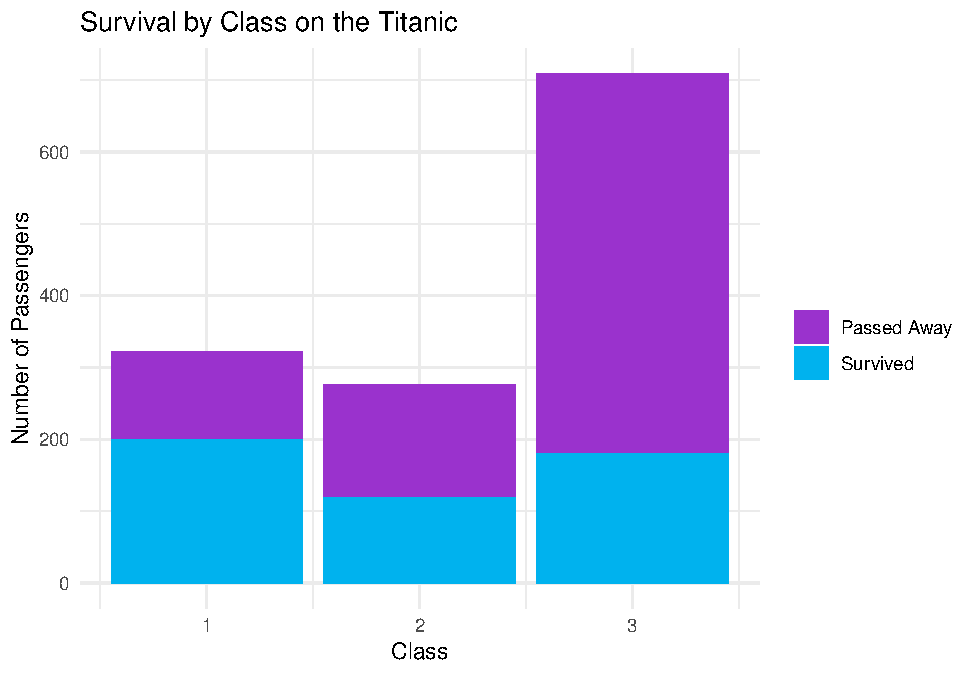
\includegraphics{README_files/figure-latex/unnamed-chunk-2-1.pdf}

This first graph gives us a visual representation of the number of
surviving passengers in different classes. As can be seen the chances of
surviving is lowest for passengers in the lowest class (third), at
slightly above 25\%. While the passengers in first class had an
approximately 62.5\% chance of survival. It should also be noted that
the number of passengers in the third class significantly outweigh the
number of passengers in the first and second class.

\hypertarget{graph-4.2}{%
\subsection{Graph 4.2}\label{graph-4.2}}

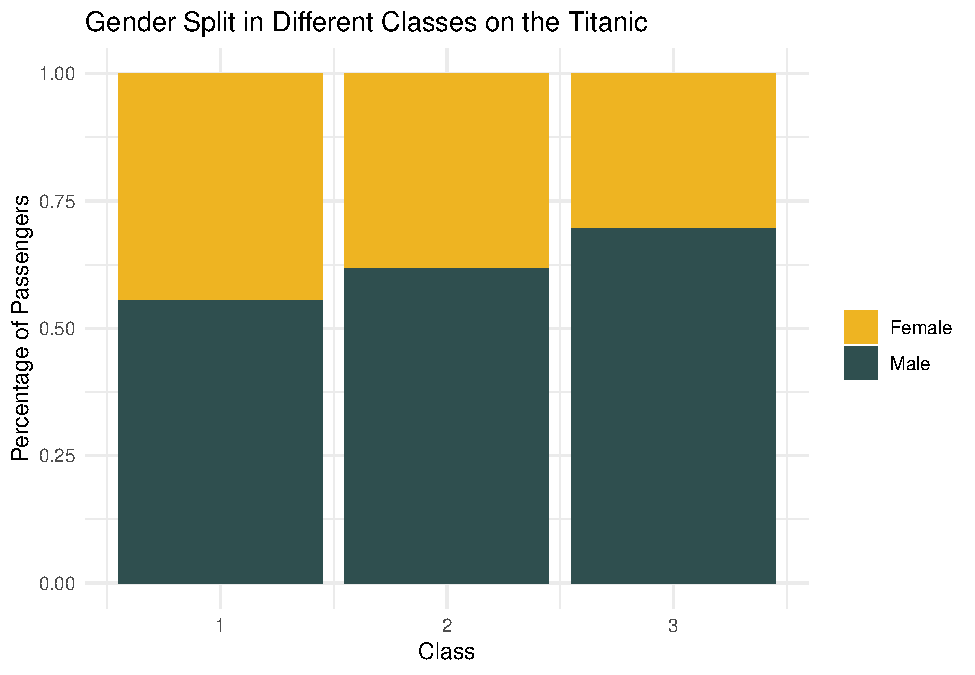
\includegraphics{README_files/figure-latex/unnamed-chunk-3-1.pdf}

It is noticeable from this graph that the percentage of men differ
between classes. With the composition becoming more male orientated the
lower the class. In the first class it is only slightly male orientated,
with 55.42\% of the passengers being male. However, in the third class
the male percentage rises to 69.53\% of the passengers.

\hypertarget{graph-4.3}{%
\subsection{Graph 4.3}\label{graph-4.3}}

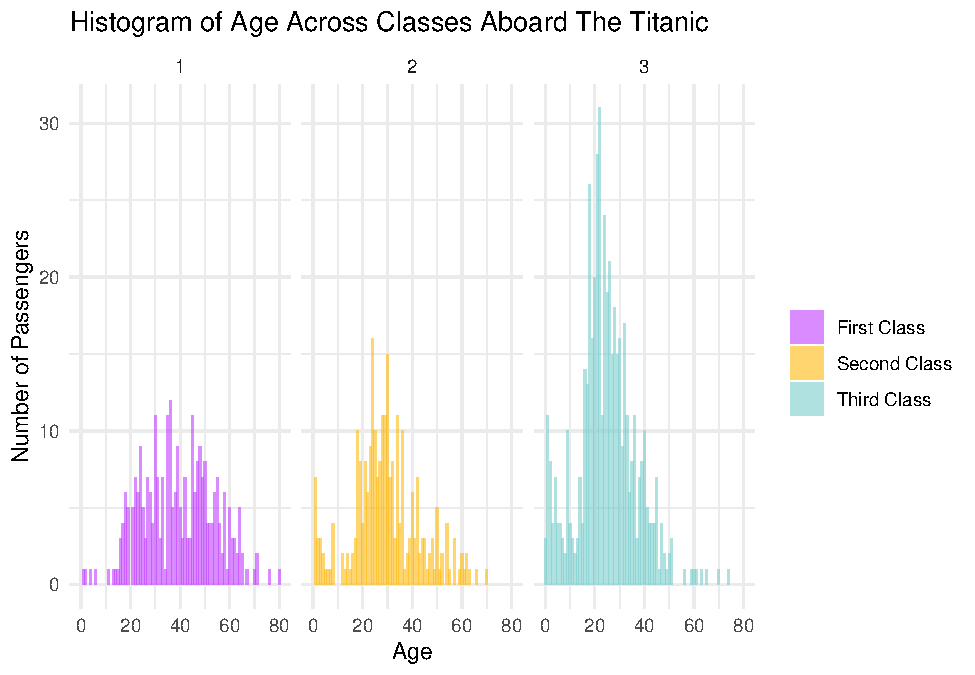
\includegraphics{README_files/figure-latex/unnamed-chunk-4-1.pdf}

Here we can see a side by side comparisons of the age compositions of
the different classes aboard the Titanic. From this comparison we can
see that the third class was composed of a higher percentage of younger
people than first or second class. With first class being the least
skewed of the three classes.

\hypertarget{graph-4.4}{%
\subsection{Graph 4.4}\label{graph-4.4}}

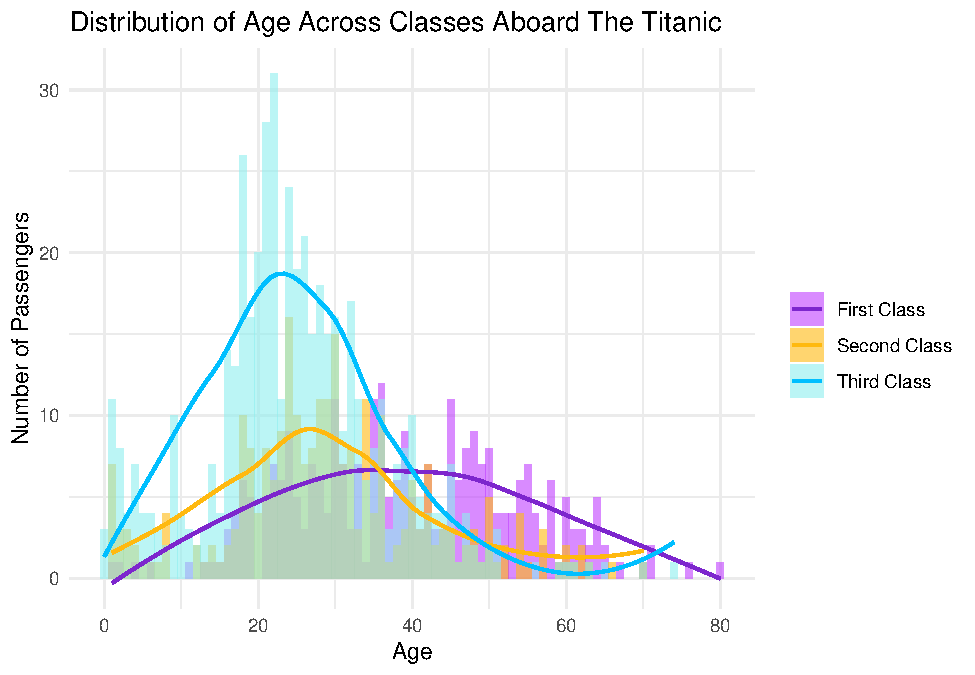
\includegraphics{README_files/figure-latex/unnamed-chunk-5-1.pdf}

\hypertarget{graph-4.5}{%
\subsection{Graph 4.5}\label{graph-4.5}}

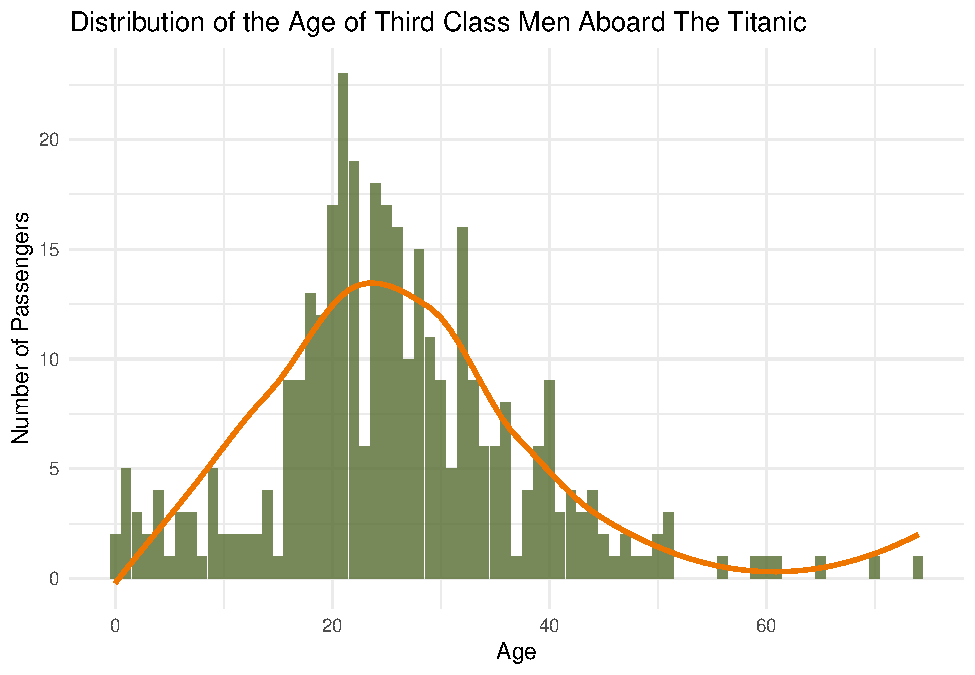
\includegraphics{README_files/figure-latex/unnamed-chunk-6-1.pdf}

\hypertarget{graph-4.6}{%
\subsection{Graph 4.6}\label{graph-4.6}}

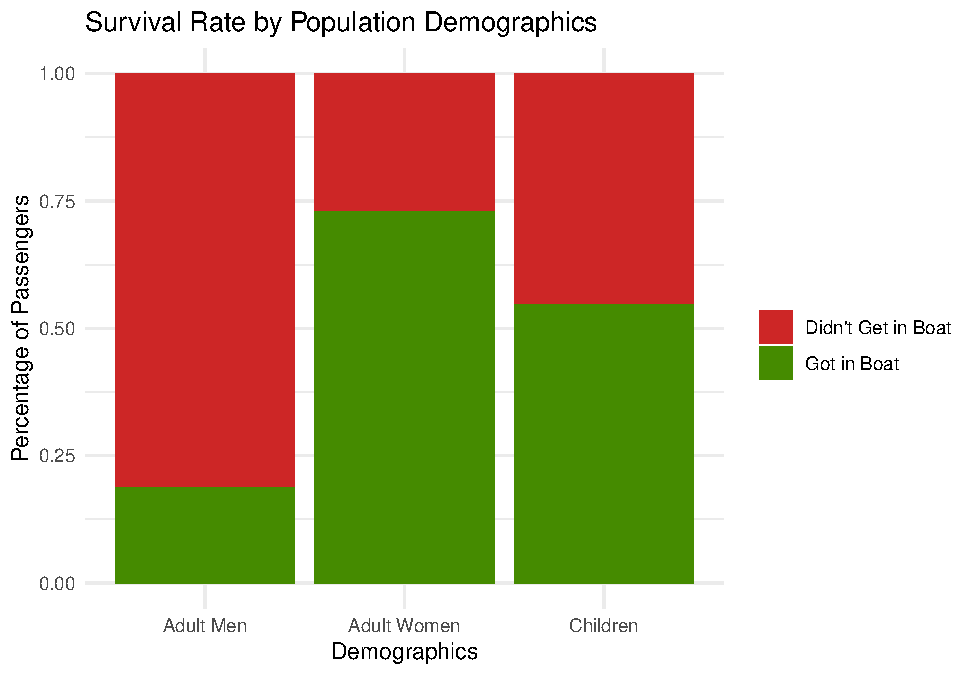
\includegraphics{README_files/figure-latex/unnamed-chunk-7-1.pdf}

\end{document}
